
%!TEX root = proposta.tex 
%% Matheus renomeia "exemplo.tex" para um nome mais descritivo (e muda a linha acima)
\chapter{\label{chap:conte}Contexto}

%\frm[inline]{Coloca um parágrafo de signposting, diz o que tu vais tratar aqui, e dá uma palha rápida de por que.}

\section{Busca adversaria}

A busca adversaria é utilizada para ambientes competitivos, como nos jogos. Como em um jogo o jogador, preferencialmente, não informa suas jogadas previamente, o ambiente se torna imprevisível, e com isso os objetivos dos jogadores entram em conflito, ambos estão em busca da vitoria. Como solução para esse problema é preciso gerar uma solução de contingencia para tentar antecipar as jogadas do adversário \cite{intelligence2003modern}. 

Para explicar como resolver esse problema, primeiro é preciso considerar um jogo com dois jogadores, um é chamado de MAX e o outro de MIN. O jogador MAX começa o jogo e o jogo e então é alternado uma jogada de MIN e uma de MAX até o final do jogo. Ao final do jogo, quem vence obtém uma recompensa positiva e quem perde uma negativa. Um jogo pode ser formalizado como \cite{intelligence2003modern}:

\begin{itemize}
	\item $S_{0}$ - O estado inicial, que especifica como o jogo se configura no inicio.
	\item Jogadores(s) -  Define qual jogador tem o movimento no estado.
	\item Ações(s) - Conjunto das ações possíveis em um estado.
	\item Resultado(s, a) - Um modelo de transição, que define o resultado da ação a aplicada ao estado s.
	\item Terminal(s) - Verifica se o estado é um estado onde o jogo terminou.
	\item Utilidade(s,p) - Define qual é o valor numérico para o jogo quando atingir um estado s terminal por um jogador p. 
\end{itemize}

O estado inicial, as ações e os resultados definem a arvore das jogadas para o jogo. A arvore representa em cada nodo um estado do jogo e cada ligação com os níveis de baixo são os estados resultantes após a execução de cada ação possíveis para o estado. A alternância entre as jogadas de MAX e MIN até chegar as folhas da arvore que correspondem aos estados terminais. Como o ponto de vista é do MAX, o valor de cada nodo folha representa o valor de utilidade para o MAX, e os maiores valores representam bons resultados para o MAX e ruins para o MIN. Com isso o caminho resultante indica que aquela ação será a melhor ação para o estado atual. 
%\msr{colocar uma figura de uma game tree?}

Este tipo de busca leva em consideração que o jogador adversário sempre realizará a jogada que mais lhe beneficiará. Um algoritmo que utiliza deste recurso é o algoritmo \textit{minimax search}.


\section{Planejamento} 
%\frm[inline]{Sempre que citar livro, dizer capítulo e páginas}
Planejamento automatizado é uma área da inteligencia artificial que estuda o processo de geração de planos de forma computacional. Este tipo de planejamento está preocupado com a forma geral da composição dos planos \cite{ghallab2004automated}. O planejamento na computação se diferencia das outras áreas pelo fato de que todo o plano é gerado automaticamente. 

Uma entrada necessária para qualquer algoritmo de planejamento é a representação do problema a ser resolvido. A representação de um problema é onde estão descritos os estados e as transições dos estados. Um estado do sistema é representados por um conjunto de átomos que resultam em verdadeiro ou falso dependendo da interpretação do ambiente. Para determinar as transições dos estados são utilizadas ações que são  representadas por operadores de planejamento que alteram os valores dos átomos presentes em determinado estado. Um operador de planejamento é definido como \textit{op} = (nome(\textit{op}), precondições(\textit{op}), efeitos(\textit{op})), onde cada elemento é definido como \cite{ghallab2004automated}: 

\begin{itemize}
	\item nome(\textit{op}) - É o nome do operador de planejamento e \textit{op} é o conjunto de todas as variáveis que irão aparecer qualquer parte do operador de planejamento.  
	\item precondições(\textit{op}) - \textit{op} é o conjunto de átomos ou átomos negativos que representa a precondição do operador de planejamento. 
	\item efeitos(\textit{op}) - \textit{op} é o conjunto de átomos ou átomos negativos que representa o efeito do operador de planejamento
\end{itemize}

O nome deve ser único pelo proposito de o nome poder se referir ao operador por completo, ou seja, após definido apenas com o nome pode-se inferir as pré e pós condições, assim escrevendo o nome(\textit{op}) para se referir a todo o operador de planejamento \textit{op}. 

Um problema de planejamento é descrito como \textit{P} = \textit{($\Sigma$, $s_{0}$, g)}. Onde $\Sigma$ é a representação do problema, $s_{0}$ é o estado inicial, estado onde o problema começa, e g é o objetivo, estado onde o problema deve acabar. Um planejador é responsável por pegar essas informações e gerar um plano que comece pelo estado inicial e chegue ao objetivo através de um conjunto de ações descritas na representação do problema. A figura \ref{fig:planmodelo} representa esse processo.

\begin{figure}[ht]
	\centering
	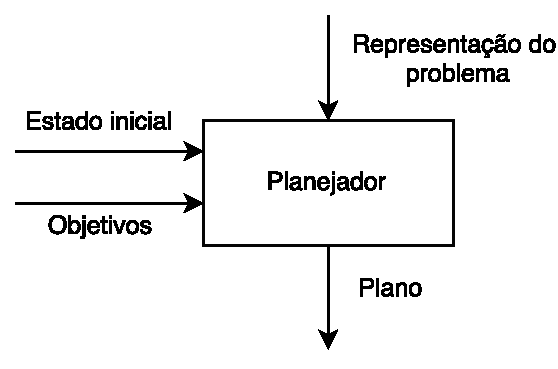
\includegraphics[width=0.4\textwidth]{fig/modelo.pdf}
	\caption{Problema de planejamento}
	\label{fig:planmodelo}
\end{figure} 


\subsection{HTN} 

Dentro da área de planejamento existe o planejamento hierárquico, chamado de \textit{Hierarchical Task Network} (HTN). HTN é igual ao planejamento clássico, quando se refere a representação do problema, entretanto o diferencial vem do que é planejado e como é planejado \cite{ghallab2004automated}, mas acaba sendo mais expressivo que o planejamento clássico, porque no planejamento clássico o conjunto de solução dos problemas é uma linguagem regular, ou seja, pode ser expressada por uma expressão regular, já em HTN dependendo da técnica utilizada o conjunto de solução dos problemas pode chegar a uma linguagem livre de contexto, que contém as linguagens regulares como um subconjunto, pois existem linguagens livres de contexto que não são linguagens regulares. No pior caso o resultado gerado do planejamento clássico será exponencialmente maior do que o gerado pelo planejamento HTN \cite{ghallab2004automated}.  

Em planejamento HTN as ações são tratadas em mais alto nível \cite{intelligence2003modern}. e o objetivo é achar um conjunto de tarefas que resolve determinado problema. Para isso, além da representação do problema, um conjunto de métodos é adicionado como entrada, onde este conjunto serve para decompor as tarefas em tarefas menores. O planejamento é feito decompondo tarefas não primitivas recursivamente até chegar em tarefas primitivas, que podem ser realizadas com um operador de planejamento \cite{ghallab2004automated}. Um método HTN é definido como \textit{m} = (nome(\textit{m}), tarefa(\textit{m}), subtarefas(\textit{m}), limitação(\textit{m})), onde cada elemento é definido como \cite{ghallab2004automated}: 

\begin{itemize}
	\item nome(\textit{m}) - Nome do método, que deve ser único, e \textit{m} é o conjunto de variaveis que será utilizado em \textit{m}. 
	\item tarefa(\textit{m}) - É uma tarefa não primitiva.
	\item (subtarefa(\textit{m}),limitação(\textit{m})) - É uma ligação de tarefa de ligação.
\end{itemize}

Uma tarefa de ligação é definida como um par w = (U,C), onde U é um conjunto de tarefas de ligação e C um conjunto de limitações. Cada limitação deve ser satisfeita em todo o plano e cada tarefa de ligação é decomposta em sub tarefas até todas as tarefas se tornarem primitivas. 

Um problema de planejamento HTN é descrito como P = ($s_{0}$, w, O, M), onde $s_{0}$ é o estado inicial, w a tarefa de ligação inicial, O é um conjunto de operadores de planejamento, e M é um conjunto de métodos. 

Na busca pelo plano, o planejamento HTN começa planejando por um caminho, quando um caminho de resolução leva a um fim de linha é realizado um retrocesso(\textit{backtracking}) até um caminho que tenha uma possibilidade diferente de caminho do que foi tomado anteriormente.


\subsection{AHTN} 

\textit{Adversarial hierarchical-task network} (AHTN) é um algoritmo proposto para tentar solucionar o problema do grande fator de ramificação dos jogos em tempo real \cite{ontanon2015adversarial}. Nele são combinados técnicas de HTN com o algoritmo \textit{minimax search}. O algoritmo \ref{alg:ahtn} é a representação da técnica de AHTN. Cada nodo da arvore das jogadas é definido por uma tupla $(s, N_{+}, N_{-}, t_{+}, t_{-})$, onde s é o estado corrente do ambiente, $N_{+}$ e $N_{-}$ são a representação de planos HTN para os jogadores max e min, respectivamente, $t_{+}$ e $t_{-}$ representam ponteiros para qual parte do plano HTN está sendo executado, sendo  $t_{+}$ uma tarefa de $N_{+}$ e $t_{-}$ uma tarefa de $N_{-}$. \textit{nextAction(N,t)} é uma função que, dado um HTN N e um ponteiro t, encontra a tarefa primitiva que deve ser executada em N. Se N ainda não estiver completamente decomposto, ou seja, ainda existem tarefas não primitivas, então \textit{nextAction(N,t)} = $\perp$.  $decompositions_{+}(s, N_{+}, N_{-}, t_{+}, t_{-})$ denota o conjunto das decomposições validas que adicionem apenas um novo método em $N_{+}$. A partir de uma função de avaliação, que pode ser aplicada sobre um estado, é retornado a recompensa de max em um estado terminal ou uma aproximação se o estado for não terminal. A partir destas definições, o algoritmo para AHTNMin é análogo. O algoritmo retorna o melhor plano encontrado para os dois jogadores, e também o resultado da função de avaliação no nodo terminal alcançado após a execução dos planos. A grande diferença entre o algoritmo de AHTN e o algoritmo do \textit{minimax search}, é que as chamadas recursivas nem sempre se alternam entre max e min. O algoritmo troca de nodos max para min apenas quando os planos estão totalmente decompostos a ponto de gerar uma ação. 

\begin{algorithm}
	\caption{AHTNMax(s, $N_{+}$, $N_{-}$, $t_{+}$, $t_{-}$, d)}
	\label{alg:ahtn}
	\begin{algorithmic}[1]
		\If {terminal(s) $\vee$ d $\leq$ 0}
		\State	\Return ($N_{+}$, $N_{-}$, e(s))
		\EndIf
		\If {nextAction($N_{+}$, $t_{+}$) $\neq$ $\perp$}
		\State t = nextAction($N_{+}$, $t_{+}$) 
		\State \Return AHTNMin($\gamma$(s,t), $N_{+}$, $N_{-}$, t, $t_{-}$, d-1)
		\EndIf
		\State $N_{+}^{*}$ = $\perp$, $N_{-}^{*}$ = $\perp$, $v^{*}$ = $-\infty$
		\State $\aleph$ = $decompositions_{+}(s, N_{+}, N_{-}, t_{+}, t_{-})$
		\ForAll{$N \in \aleph$}
		\State $(N^{'}_{+}, N^{'}_{-}, v^{'}) = AHTNMax(s, N, N_{-}, t_{+}, t_{-}, d)$
		\If{$v^{'} > v^{*}$}
		\State $N_{+}^{*} = N^{'}_{+}, N_{-}^{*} = N^{'}_{-}, v^{*} = v^{'} $
		\EndIf
		\EndFor		
		\State \Return $(N_{+}^{*}, N_{-}^{*}, v^{*} )$
	\end{algorithmic}
\end{algorithm}



\section{Aprendizado} 
Para os humanos o aprendizado ocorre durante toda a vida. 
O aprendizado é o ato de adquirir novos conhecimentos, ou modificar conhecimentos já existentes ou ainda adquirir uma experiencia por repetição do ato de forma incorreta. 
Aprendizado pode variar de adquirir conhecimento de tarefas simples, como decorando um numero de telefone, até tarefas mais complicadas, como a formulação de novas teorias \cite{intelligence2003modern}. 
% Não precisa colocar quebra de parágrafo em todo o lado!

\subsection{Aprendizado de Máquina} 

A área na computação que estudo esse aprendizado de forma computacional é o aprendizado de maquina, melhor conhecida como \textit{machine learning}. A definição de aprendizado de maquina proposta por Tom Mitchell \cite{Mitchell1997ML} é a seguinte:

\begin{quote}
	Definição: Um programa de computador é dito que aprende de uma experiencia E com relação a alguma classe de tarefas T, e medida de performance P, se essa performance sobre as tarefas em T, medida por P, melhora com a experiencia E.
\end{quote}

Essa definição mostra que o sistema aprimora seu conjunto de tarefas T com uma performance P através de experiencias E. Ou seja, um sistema baseado em aprendizado de maquina deve, através de experiencias, ter um ganho nas informações para solucionar os seus problemas. Para começar a resolver um problema utilizando aprendizado de maquina é preciso escolher qual experiencia será aprendida pelo sistema \cite{Mitchell1997ML}. Para isso existem algumas técnicas que tratam aprendizado de maquina com objetivos diferentes \cite{intelligence2003modern}. Alguma das técnicas são: %\frm{Olha as concordâncias!!}

%\frm[inline]{Escrever sentenças completas!}
\begin{itemize}
	\item Aprendizado supervisionado: Aprender através de algum conjunto de exemplos a realizar a classificação de algum problema. Cada problema é mapeado para uma saída. 
	\item Aprendizado não supervisionado: Aprender através das observações, algum pedrão ou regularidade, para classificar em grupos os problemas.
	\item Aprendizado por reforço: Aprender através das execuções, bem ou mal sucedidas. Aprende quais ações são melhores de ser executadas.
\end{itemize}

%\frm[inline]{Reescrever tudo isto, e organizar os pensamentos. Onde tu queres chegar com o parágrafo?}


O aprendizado por reforço também é conhecido como \textit{reinforcement learning}. O objetivo deste aprendizado é usar as recompensas obtidas nas observações para aprender uma politica do ambiente \cite{intelligence2003modern}. Para que isso aconteça, cada estado contém uma utilidade, que mostra o quão desejável é este estado, pode ser um desejo bom ou um ruim. Com essa informação é possível determinar, dado as ações disponíveis no estado, qual ação o sistema deve escolher para seguir a execução. 


%O aprendizado por reforço, também é conhecido como \textit{reinforcement learning}, \textbf{tem as técnicas }\frm{ARGH!!!} baseadas em  aprender através das execuções e a cada nova execução o conhecimento aprendido é utilizado para tentar maximizar o seu desempenho na próxima execução \cite{intelligence2003modern}. Para conseguir medir o aprendizado em cada execução, existe a abordagem que é preciso medir a quantidade do ganho por estado do sistema e assim cada estado do sistema deve ter um valor de utilidade para dizer se o estado é um estado recomendado ou não para ser alcançado, ou ainda o estado não oferece nem ganho nem perda por ser atingido. 


\section{Jogos Real-time Strategy(RTS)} 

Jogos eletrônicos são muito populares, principalmente pela grande quantidade de gêneros, existem jogos de ação, aventura, esportes, estrategia, entre outros. Dentro dos jogos de estratégia há uma subseção que se chama jogos de estratégia em tempo real, neles os jogadores estão se enfrentando no mesmo momento, como o nome já diz. \\

Um exemplo deste gênero é o Starcraft\footnote{http://us.battle.net/sc2/pt/}.  Uma simplificação do Starcraft foi feita por Santiago Ontañón \cite{ontanon2013combinatorial}, chamada de MicroRTS. O MicroRTS foi desenvolvido para fins acadêmicos, com o intuito de aplicar e desenvolver técnicas de IA e para servir como prova de conceito para as técnicas criadas.  O objetivo do jogo é destruir a base adversaria. Existem trabalhadores que podem coletar recursos e construir outros prédios. Os recursos são coletados dos minerais. Com os recursos é possível construir bases de ataque, onde são realizado o treinamento de unidades de ataque. Para conseguir realizar o objetivo de destruir a base adversaria é preciso ter unidades de ataque. O jogo oferece três destas unidades, são elas:

\begin{itemize}
	\item Heavy - Possui um alto poder de ataque, mas sua velocidade é lenta.
	\item Light - Possui um baixo poder de ataque, mas sua velocidade é rápida.
	\item Ranged - Possui um ataque de longa distancia. 
\end{itemize} 

A Figura~\ref{fig:microrts}\footnote{https://github.com/santiontanon/microrts} mostra uma tela do jogo que representa o que foi explicado e ainda é possível observar que o fator de ramificação pode ser muito alto dependendo do cenário do jogo. %\frm{Figura sem explicação... Só os comentários do lado, em inglês, não te resolvem}

\begin{figure}[ht]
	\centering
	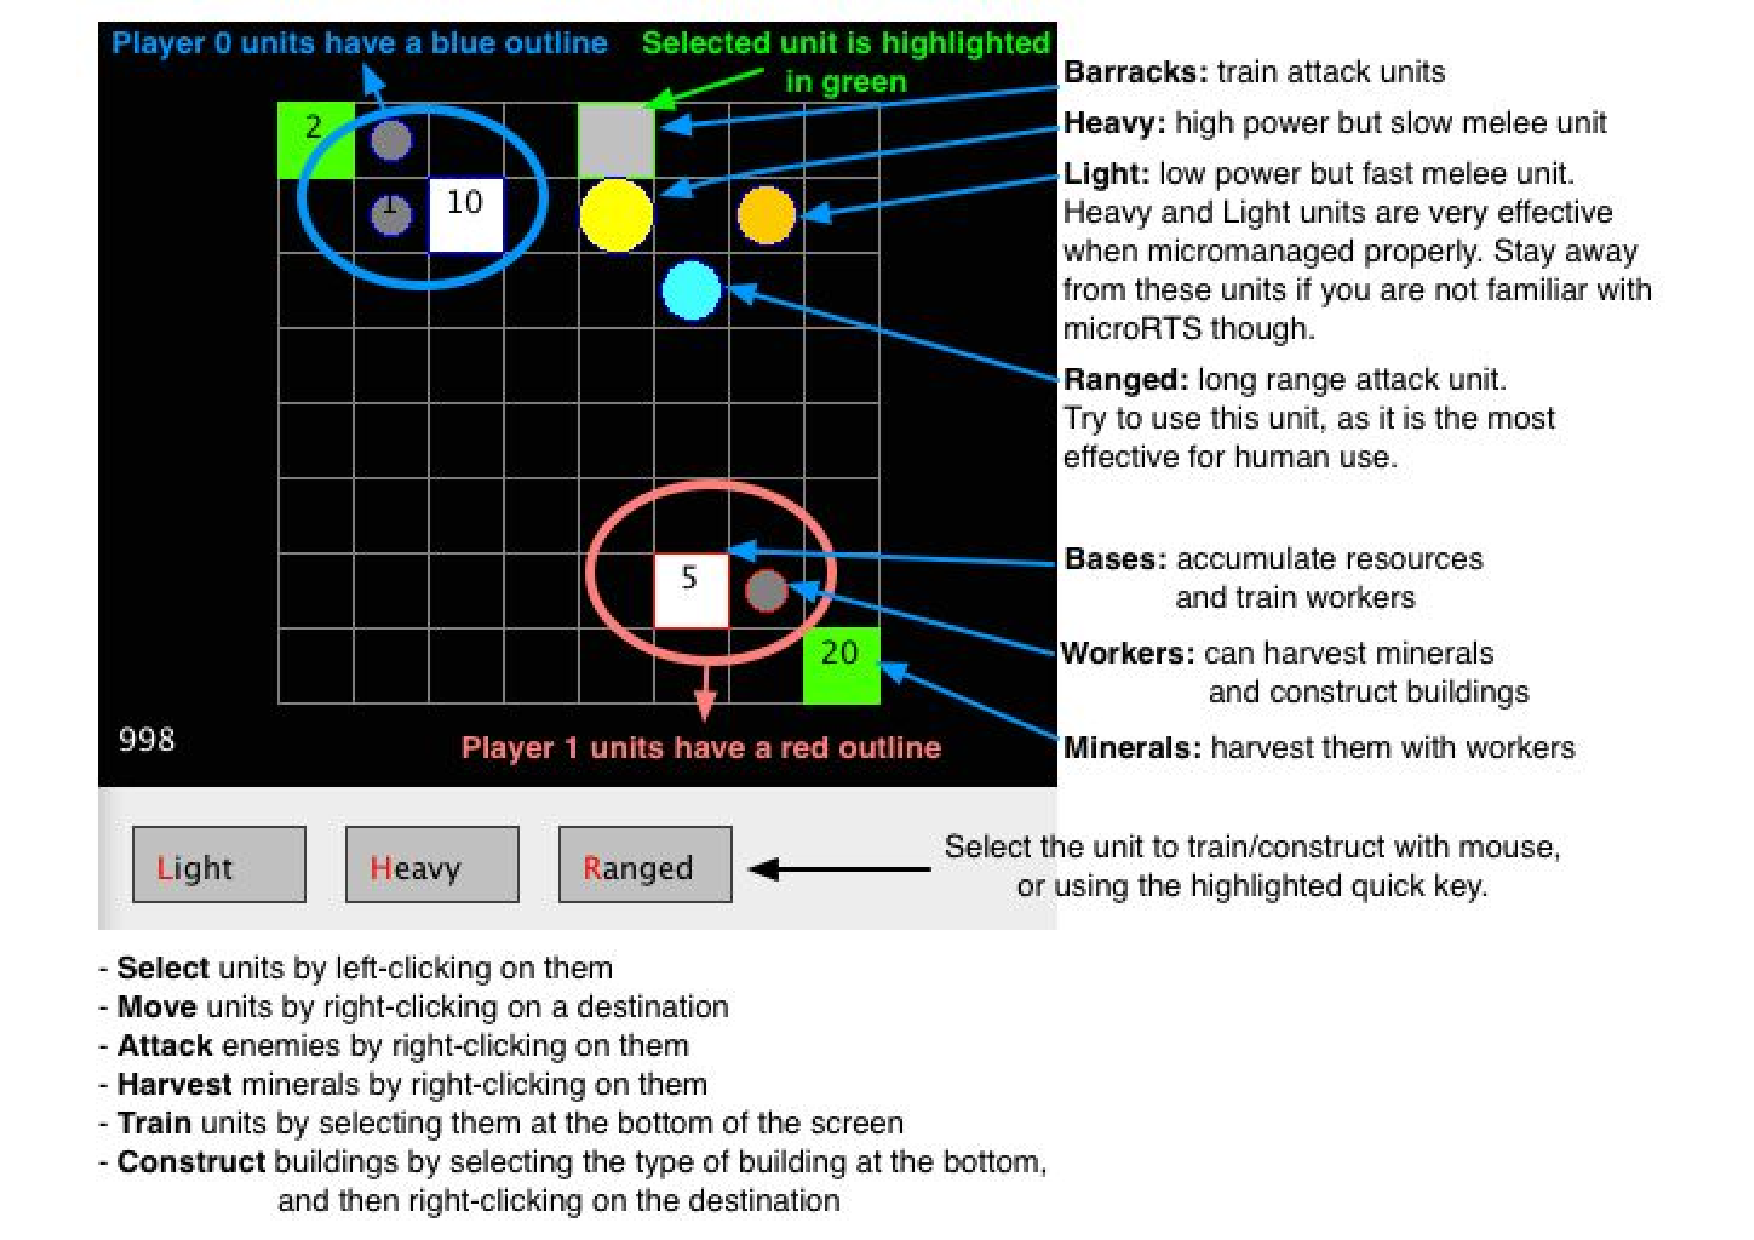
\includegraphics[width=0.5\textwidth]{fig/microrts.pdf}
	\caption{Um exemplo da tela do MicroRTS}
	\label{fig:microrts}
\end{figure} 

No ambiente há algumas estrategias implementadas, cada estrategia possui variações dos algoritmos. Algumas das estrategias são:
\begin{itemize}
	\item Minimax Alpha-Beta Search Strategies - O que muda entre as técnicas é o jeito com que é feito a expansão do grafo.
	\item Monte Carlo Search Strategies - Executa jogadas aleatórias para planejar e após utiliza uma heurística para determinar em qual caminho seguir.
\end{itemize}

%\frm[inline]{E.. depois da itemização talvez seja interessante concluir algo}
A plataforma já foi utilizada para aplicar técnica de IA. Por esse motivo a utilização desta plataforma se torna viável. A comparação entre as estrategias já existentes com a que estou propondo pode mostrar que a abordagem resulta em um melhor desempenho. 



